\documentclass[12pt]{article}

\title{A note on anisotropic quantum gravity}
\author{S. Halayka\footnote{sjhalayka@gmail.com}}
\date{\today\;\currenttime}

\usepackage{datetime}
\usepackage{listings}
\usepackage{cite}
\usepackage{xcolor}
\usepackage{graphicx}
\usepackage{setspace}
\usepackage{amsmath}
\usepackage{url}
\usepackage[margin=1in]{geometry}
%\doublespace



\begin{document}



 
\maketitle

\begin{abstract}
In Newton's theory, all mass gravitates in an {\textit{isotropic}} (spherical) manner.
In this paper, we will consider aspherical -- {\textit{anisotropic}} -- gravitating processes, which leads to a unique view of dark matter: dark matter is a graviton condensate.
We also discuss dark energy, and the possibility of a final, $5$th interaction.
\end{abstract}





\section{Introduction}

This paper is based on one main assumption: the gravitational field is {\textit{quantized}} into {\textit{gravitons}}.
Unfortunately, we have no empirical evidence that gravitons actually exist, although superstring theory \cite{wray} does predict such a particle.
We try to make the best of the situation, as we lay out 7 sections on what quantum gravity would actually be like.
In these sections we interpret the following topics using the paranoiac critical method:
\begin{itemize}
\item Time dilation at a high level
\item Anti-gravity and time contraction
\item The holographic principle and the gravitational keystone
\item Information retention
\item Gravitational time dilation at a mid level
\item Dark matter, and fractional dimensions that follow a power law
\item Dark energy, length dilation, and the accelerating expansion of the Universe
\end{itemize}

Finally, we present a review of the discussion.

%Please note that this paper uses colloquial language, made for and by the layman.







\section{On the interruption of a process by time dilation}

A {\textit{process}} is a system of mass-energy, including its internal interactions, over time.

Time dilation is the {\textit{interruption}} of said process, whether it be kinematic and/or gravitational -- both are the result of external interactions.
In the case of the gravitational interaction, the process is interrupted by spacetime itself (e.g. gravitons).
In the case of the non-gravitational interaction, the process is interrupted by the other particles (e.g. photons, etc).

This gravitational time dilation \cite{misner} is encoded in the first term on the right-hand side of the Schwarzschild line element in Einstein's general relativity
\begin{equation}
ds^2 = -\left( 1 - \frac{R_s}{r} \right) c^2 dt^2 + \frac{dr^2}{\left( 1 - \frac{R_s}{r} \right)} + r^2 (d\theta^2 + \sin^2 \theta d\phi^2),
\end{equation}
where $R_s$ is the Schwarzschild radius
\begin{equation}
R_s = \frac{2GM}{c^2},
\end{equation}
and $M$ is the mass of the gravitating process.
Note that the Schwarzschild line element is irrotational -- it is used here as a rough model, useful for where rotation speed is practically zero (when compared to the speed of light).

Simplified, the gravitational time dilation equation is based on distance $r$:
\begin{equation}
dt' = dt \sqrt{1 - \frac{R_s}{r}},
\end{equation}
and the kinematic time dilation equation is based on speed $v$:
\begin{equation}
dt' = dt \sqrt{1 - \frac{v^2}{c^2}}.
\end{equation}
The closer you are to a gravitating process, the slower your rate of time.
Likewise, the faster you go, the slower your rate of time.
In conjunction, this gravitational and kinematic time dilation produces an experimentally verified relativistic perihelion shift in the planets, for example.

In essence, a process {\textit{blossoms}} as time dilation increases, opening up like a flower in the sunlight as internal interaction is overcome by external interaction.
As a process falls toward a black hole's event horizon, the process is interrupted to the point where it becomes fully {\textit{assimilated}} -- it becomes one process with the black hole.

If all of physics is about processes, then it is therefore all about {\textit{computation}} \cite{zuse, wolfram} -- here we have even adopted the concept of process interruption, which is surely familiar to all x86 assembly programmers \cite{abrash}.







\section{On anti-gravity and time contraction}

%It should be noted that there is no {\textit{anti-gravity}} -- there is no {\textit{anti-interruption}, just simply a {\textit{lack}} of interruption.
%That said, 
There is the {\textit{overclocking}} and {\textit{optimization}} of processes to consider -- literally making a process run faster than its natural rate by reducing redundant and slow interactions \cite{wainner, mcconnell, pikus}.
That is, there is the possibility of time {\textit{contraction}}, and {\textit{anti-gravity}}.






\section{On taking the holographic principle literally}

In simple terms, the holographic principle states that a black hole process is the {\textit{densest}} process for any given mass $M$ -- contemporary digital or quantum processors are nowhere close to this limit.

It takes $n$ Boolean degrees of freedom (e.g. a measurement of binary entropy, also known as information) to describe the gravitational field \cite{hooft, susskind, bousso} generated by a Schwarzschild black hole process of mass $M$.
Where $M_p^2 = \hbar c / G$ is the Planck mass squared, this number of gravitational degrees of freedom is
\begin{equation}
%n = \frac{A_s}{4 \ell_p^2 \log(2)},
n = \frac{4\pi M^2}{ \log(2) M_p^2}.
\end{equation}
%where in the case of the Schwarzschild line element, the event horizon area is
%\begin{equation}
%A_s = 4 \pi R_s^2.
%\end{equation}
Note that where the mass is less than the Planck scale, the process is a normal particle.
Otherwise, where the mass is equal to or greater than the Planck scale, the process is a black hole.

In effect, the black hole event horizon is quantized -- the event horizon is made up of an ensemble of $n$ Planck-scale oscillators.
All of the non-gravitational degrees of freedom have been stripped away as gravitational waves, leaving only the gravitational degrees of freedom.
In other words: a black hole is raw spacetime.

In this paper we take the holographic principle literally, and so even for non-black hole processes, the number of gravitational degrees of freedom is still $n$ -- the process is just not as small as a black hole would be.
Of course, the non-black hole also contains non-gravitational degrees of freedom, something that the black hole process does not.

It's a matter of minimum size -- there is no {\textit{singularity}} in this model of the black hole process.
In effect, each of the $n$ oscillators act as a {\textit{keystone}}, stopping one another from falling further toward the centre of the black hole process.







\section{On the retention of information}

As for information loss (e.g. $dn / dt < 0$), there must be none, due to the $2$nd law of thermodynamics.
The Hawking black body radiation that escapes the gravitation of the black hole process must carry away information, where the corresponding Schwarzschild radius is
\begin{equation}
%R_s = \frac{4 \pi G \hbar f}{c^4},
R_s = \frac{4 \pi \ell_p^2 f}{c},
\end{equation}
and $f$ is the photon frequency.
The maximum frequency is the Planck frequency
\begin{equation}
f_p = \frac{1}{2 \pi} \sqrt{\frac{c^5}{\hbar G}}.
\end{equation}
The number of gravitational degrees of freedom is
\begin{equation}
%n = \frac{16 \pi^3 \hbar G f^2}{c^5 \log(2)},
n = \frac{4 \pi f^2}{\log(2) f_p^2}.%,
\end{equation}
%where $n \leq 4\pi/\log(2)$, and $4\pi/\log(2) = 18.13$.
All but Planck-scale photons have less than $1$ gravitational degree of freedom, and so it must take an entire electromagnetic field to encode many gravitational degrees of freedom at once.

%\begin{equation}
%n = \frac{k 16 \pi^3 G \hbar f^2}{c^5 \log(2)}.
%\end{equation}
%When using geometrized units, this simplifies to
%\begin{equation}
%n = \frac{16 \pi^3 f^2}{\log(2)},
%\end{equation}
%and so it becomes readily apparent that the maximum value for $f$ is the Planck frequency.











\section{On the mechanism behind gravitational time dilation}
It's important to note that there is no such thing as a gravitational {\textit{shadow}}.
This means that all mass {\textit{relays}} (e.g. {\textit{repeats}}) all gravitons, which allows a gravitating process to {\textit{indirectly}} influence even more than $n$ receivers.
It also means that a process is interrupted by the act of relaying itself -- the relaying of gravitons is the source of gravitational time dilation.
%Thus, there is a fundamental limit to the amount of processing that can occur per unit of time, otherwise the relaying of gravitons would not cause time dilation at all.

In effect, gravity is {\textit{viral}} -- it highjacks a process, and steals cycles in order to propagate, precisely like a digital computer virus.
The closer you are, the more infected you become.
This is not to say that gravitons are alive.
Here we define life as anything that does not always follow a spacetime geodesic: birds fly, trees rise tall, and biological viruses swim.
Gravitons are taken to always follow a spacetime geodesic, and so the gravitons are not alive by our definition of the word.

With regard to a thought experiment, consider a set of jugglers.
Each juggler can only juggle so many balls per second (internal interaction).
Once the jugglers start passing balls to each other (external interaction), the number of balls juggled among their own selves (internal interaction) will reduce.
At some point the passing of balls (external interaction) could completely overcome any balls juggled among their own selves (internal interaction), where $dt'/dt = 0$.
Jugglers can only act so fast. 
In other words, the processing speed of matter is finite, and it is interruptible.




\section{On dark matter and the fractional dimension of gravitationally bound processes}

Here we use a rough model, which assumes that the gravitation is Newtonian -- irrotational like with the Schwarzschild line element, but where the gradient of time dilation has a length of practically zero (e.g. where $r \gg R_s$), and so only space is curved.

With regard to the flat rotation curve found in galactic dynamics \cite{binney}: if $n$ is at least conserved as a gravitationally bound process (e.g. the Milky Way Galaxy) goes from sphere to disk as distance from the process centre increases, then the gravitation becomes anisotropic, strengthening along the orbit plane, weakening elsewhere.
%In fact, gravitation is anisotropic for all gravitationally bound processes, for there is no such thing as a perfect spherically symmetric, isotropic, homogeneous process (not even a Schwarzschild black hole is perfectly spherically symmetric, because the event horizon is quantized).
This includes galaxies, clusters, walls, and filaments.

For a perfect sphere, the interaction strength is like $1$ with a long-range falloff proportional to $1/r^x$ where $x = 2$.
For a perfect disk, the interaction strength increases by a factor of $c$ with a long-range falloff proportional to $1/r^x$ where $x = 1$.
For a perfect filament it increases by a factor of $c^2$ with a long-range falloff proportional to $1/r^x$ where $x = 0$ (e.g. no falloff).
For these perfect shapes, the spatial dimension of the gravitational field goes from being $D = 3$ down to $D = 2$ or $D = 1$.

As for a practical application, we shall discuss a toy model of the Milky Way where the disk mass is simply taken to be zero.
It is found that at a distance of roughly $10$ kiloparsecs from the centre of the Milky Way, the spatial dimension of the gravitational field is roughly at least $D = 2.98$.
The equations used to obtain this measure are likely familiar to researchers of the fractal geometry of nature \cite{mandelbrot}:
\begin{equation}
v_n = \sqrt{\frac{GM}{r}},
\end{equation}
\begin{equation}
D = 3 - \frac{\log \left(\frac{v}{v_n} \right)}{\log(c)}
\end{equation}
\begin{equation}
v = v_n c^{3 - D},
\end{equation}
where $M = 1 \times 10^{41}$ is the mass of the Milky Way's core, $v = 220000$ is the desired circular orbit speed, and the orbit radius is $r = 3 \times 10^{20}$ metres (e.g. roughly $10$ kiloparsecs).
In general, where $D < 3$, the value of the dimension will actually be a little bit greater than that given by Eq. 10, since the falloff exponent is $x < 2$.
As such, $D$ is the minimum required value (e.g. the lower bound).
Note that $v$ changes in meaning as ${3 - D}$ increases beyond $0$, as per simple dimensional analysis.
Also note that we do not set $c = 1$, simply because to do would be to eliminate any scale-free behaviour, and cause a division by zero in Eq. 10 -- a sign that geometric units are inherently problematic when it comes to describing the scale-free reality.




%To compare with the past literature, where $v = v_n = \sqrt{GM/r} = 149157$, it is found that $D = 3$ exactly (e.g. where Newton's isotropic theory of gravitation still closely applies).
Note that where $D = 3$ is held constant, one can calculate the upper bound of the amount of dark matter:
\begin{equation}
M_{total} = \frac{r v^2 c^{2D - 6}}{G} = \frac{r v^2}{G},
\end{equation}
\begin{equation}
M_{dark} = \frac{r v^2}{G} - M.
\end{equation}
That is, the condensation of the gravitons produces a measurable amount of dark matter: at the very most $M_{dark}$.
The views that $M_{dark} > 0$ and $D < 3$ are both correct at the same time -- they are complimentary ways of describing the same thing: anisotropic gravitation leads to dark matter, which leads to anisotropic gravitation, etc.
%Numerical simulation is underway.

Here we have defined a unique view of dark matter, which forms due to anisotropic gravitation in gravitationally bound processes.
Of greatest importance is the fact that there is a finite number of gravitational degrees of freedom $n$ for a process of mass $M$, and that when aligned, these gravitational degrees of freedom form gravitational bonds that are stronger than those predicted by Newton's isotropic theory of gravitation.
Dark matter is a graviton {\textit{condensate}}.
If dark matter is a condensate of {\textit{gravitating} gravitons (e.g. gravitons that emit gravitons), then it is like the ants and their attractive, slowly evaporating, ultimately self-reinforcing pheromone trails -- that is, complex, emergent network structure occurs at the Galactic scale and larger, where gravitation is practically the only binding force.
It's impossible to deny: the simulated Universe looks very much like ant trails, biological neural networks, and wide area computer networks -- the similarity is {\textit{not}} coincidental.
The rich get richer, so to speak \cite{mm}, when it comes to forming a scale-free network in the cosmos, just like it does with ant colonies, brains, and the Internet.
See Figs. 1, 2, and 3.

It should be noted that for processes bound by all four known interactions (e.g. gravity, weak, electromagnetic, and strong), such as protoplanetary disks, there is practically no dark matter to be found, because the emission of gravitons is so very close to being isotropic due to the isotropic nature of the other three interactions.
For the Solar system -- which was once a protoplanetary disk -- the overall mass distribution has become too sparse to form any appreciable amount of anisotropic gravitation in the Sun.
This is to say that Newton's isotropic theory of gravitation still very closely applies, for the relatively small AU-scale cases where dark matter practically need not be factored in.





\section{On dark energy and the computational efficiency of the Universe}

We can only contemplate that, for the sake of symmetry in the interactions, there is a final, $5$th interaction that is even stronger than the strong interaction.
If this symmetry exists, then this $5$th interaction would be opposite of 3-dimensional gravity.
In other words: where the strong interaction is 2-dimensional (e.g. a triangle of quarks), the $5$th interaction would be 3-dimensional (e.g. a tetrahedron of constituents).
Where the strong interaction relies on 1-dimensional strings to communicate, the $5$th interaction would rely on 2-dimensional membranes.
Where the strong coupling constant is like $1$, the coupling constant for this $5$th interaction would be like $c$.

%If this $5$th interaction exists, then does it require 2 new compact dimensions in superstring theory?

Perhaps this $5$th interaction is the force behind the accelerating cosmic expansion.
If so, then time contraction is the high-level mechanism behind this $5$th interaction.
It seems that the computational efficiency of the Universe is increasing over time in general, because of the $2$nd law of thermodynamics, thus causing this time contraction (e.g. length dilation); this antithesis of gravity.



%It surely seems so, anyway.
%Would there be 3 large + 8 small spatial dimensions, plus 1 temporal dimension, adding up to 12 dimensions altogether?

%If so, is the specific non-gravitational entropy (e.g. non-gravitational entropy divided by mass) a sign of this computational efficiency?
%If so, then a black hole is indeed the most computationally efficient process for any given mass $M$, as previously mentioned in the section on the holographic principle.




\section{Review}

Evidently, time dilation exists, and so should time contraction.
We have taken the holographic principle literally, and so a mass always contains all of its gravitational degrees of freedom: $n \propto M^2$.
There was no information loss found: $dn/dt \geq 0$.
We then discussed how gravitational time dilation is caused by the relaying of gravitons.
Next we discussed dark matter, and how the gravitational interaction increases in strength when the gravitational degrees of freedom align to become oblate (e.g. 2-dimensional) or prolate (e.g. 1-dimensional).
To finish, we discussed dark energy, and a final, $5$th interaction. 

The following is a table of interactions, according to this model:
\begin{center}
\begin{tabular}{| l | r | r |}
  \hline
  Type & Inherent spatial dimension & Communication spatial dimension \\
\hline
\hline
Gravitation (isotropic) & 3  & 4\\
Gravitation (oblate) & 2 & 3\\
Gravitation (prolate) & 1 & 2\\
Weak & 0 & 1\\
Electromagnetism & 1 & 0 \\
Strong & 2 & 1\\
$5$th interaction & 3 & 2 \\
  \hline  
\end{tabular}
\end{center}

If this model is correct, then it goes to retrodict the entire dark sector.

%It appears that spacetime is at least $(4 + 1)$-dimensional.
%This many dimensions are needed in order to support a communication spatial dimension of $4$ in isotropic gravitation.




\pagebreak




\begin{thebibliography}{9}

\bibitem{wray} Wray. An Introduction to String Theory. (2011)
\bibitem{misner} Misner et al. Gravitation. (1970)
\bibitem{zuse} Zuse. Calculating Space. (1969)
\bibitem{wolfram} Wolfram. A New Kind of Science. (2002)
\bibitem{abrash} Abrash. Michael Abrash's Graphics Programming Black Book. (1997)
\bibitem{wainner} Wainner et al. The Book of Overclocking: Tweak Your PC to Unleash Its Power. (2003)
\bibitem{mcconnell} McConnell. Code Complete. 2E. (2004)
\bibitem{pikus} Pikus. The Art of Writing Efficient Programs: An advanced programmer's guide to efficient hardware utilization and compiler optimizations using C++ examples. (2021)
\bibitem{hooft} `t Hooft. Dimensional reduction in quantum gravity. (1993)
\bibitem{susskind} Susskind. The World as a Hologram. (1994)
\bibitem{bousso} Bousso. The holographic principle. (2002)
\bibitem{binney} Binney et al. Galactic Dynamics. Second Edition. (2008)
\bibitem{mandelbrot} Mandelbrot. The Fractal Geometry of Nature. (1982)
\bibitem{mm} Mitchell. Complexity: A Guided Tour. (2009)





%\bibitem{berger} Berger et al. Snowmass 2021 White Paper: Cosmogenic Dark Matter and Exotic Particle Searches in Neutrino Experiments. (2022)
%\bibitem{aalbers} Aalbers et al. First Dark Matter Search Results from the LUX-ZEPLIN (LZ) Experiment. (2022)
%\bibitem{quiskamp} Quiskamp et al. Direct Search for Dark Matter Axions Excluding ALP Cogenesis in the 63-67 micro-eV Range, with The ORGAN Experiment. (2022)
%\bibitem{haipeng} Haipeng et al. Direct detection of dark photon dark matter using radio telescopes. (2022)
%\bibitem{hui} Hui et al. Ultralight scalars as cosmological dark matter. (2016)
%\bibitem{ackerman} Ackerman et al. Dark Matter and Dark Radiation. (2008)



\end{thebibliography}


\pagebreak


\begin{figure} 
\centering
  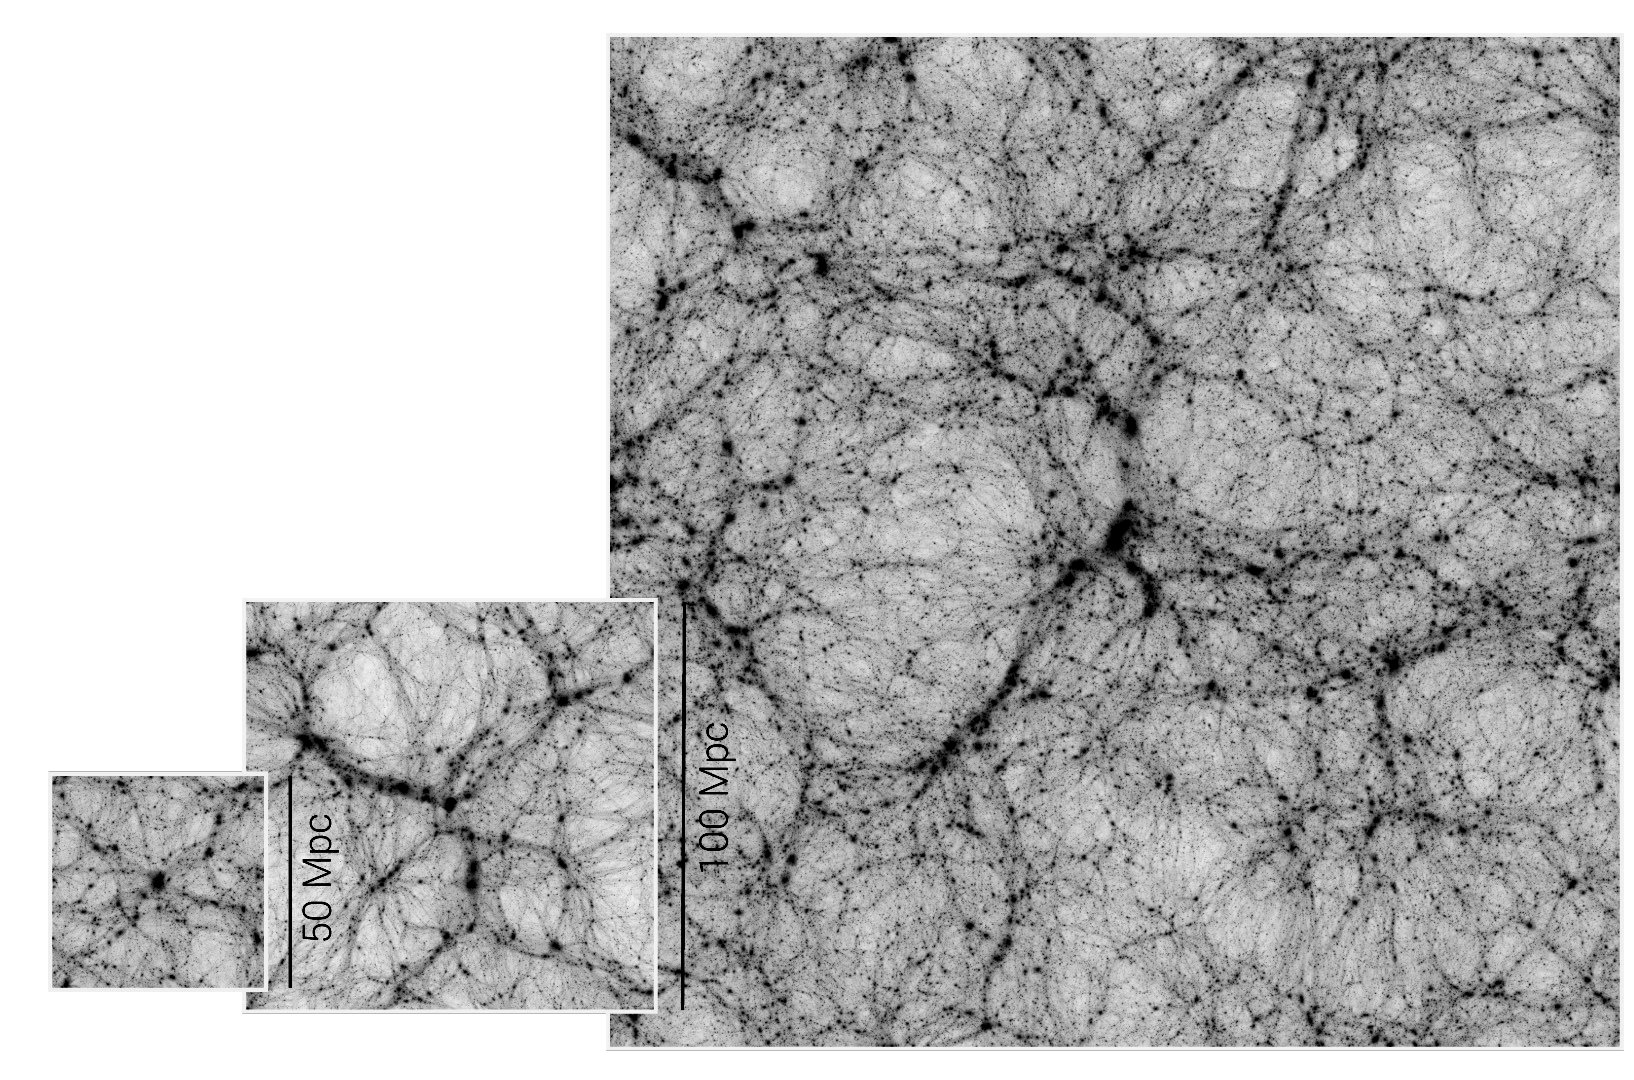
\includegraphics[width = 2 in]{TNG.png}
  \caption{ Image of Universe simulation by IllustrisTNG -- https://www.tng-project.org/
}
\end{figure}

\begin{figure} 
\centering
  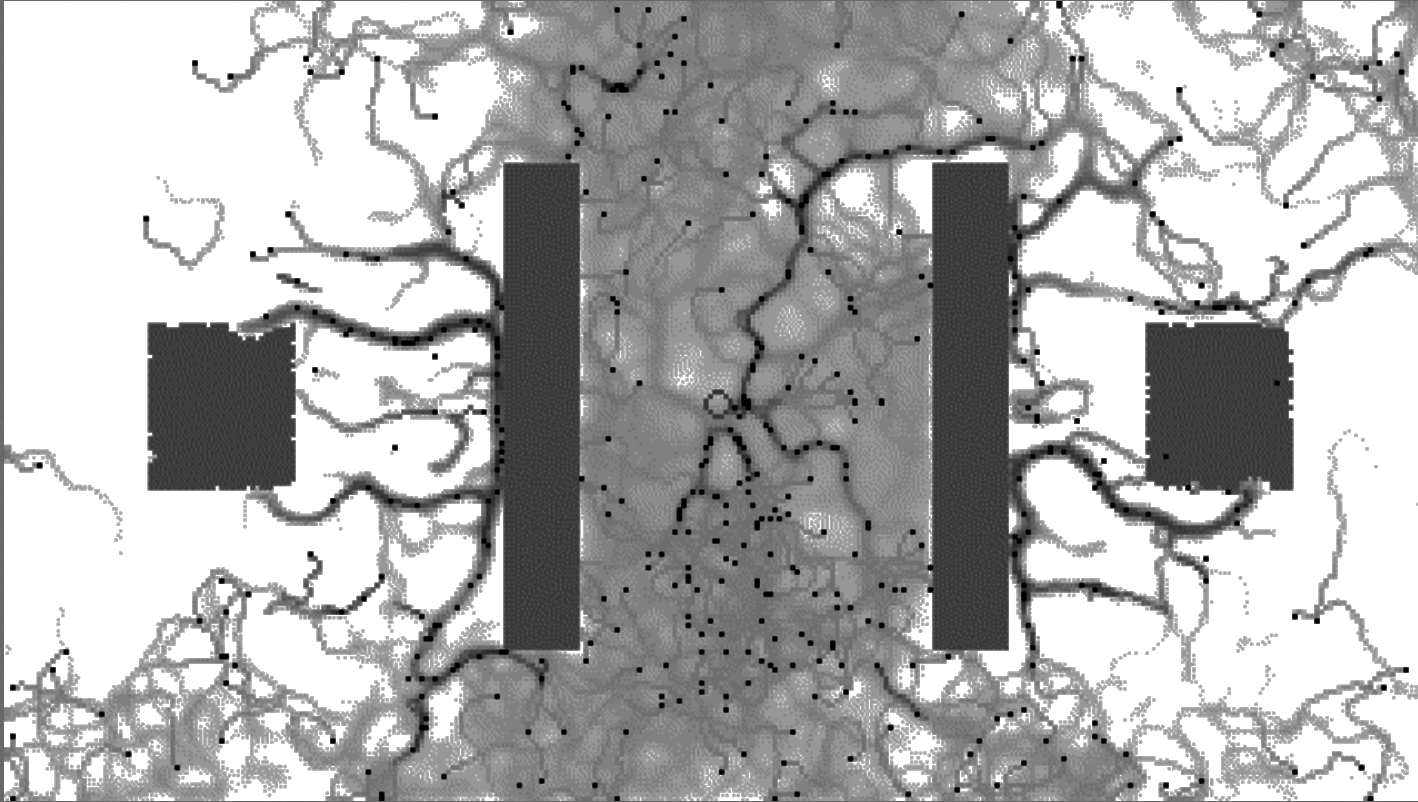
\includegraphics[width = 4 in]{ants.png}
  \caption{ Image of simulated ant trails -- https://softologyblog.wordpress.com/2020/03/21/ant-colony-simulations/
}
\end{figure}

\begin{figure} 
\centering
  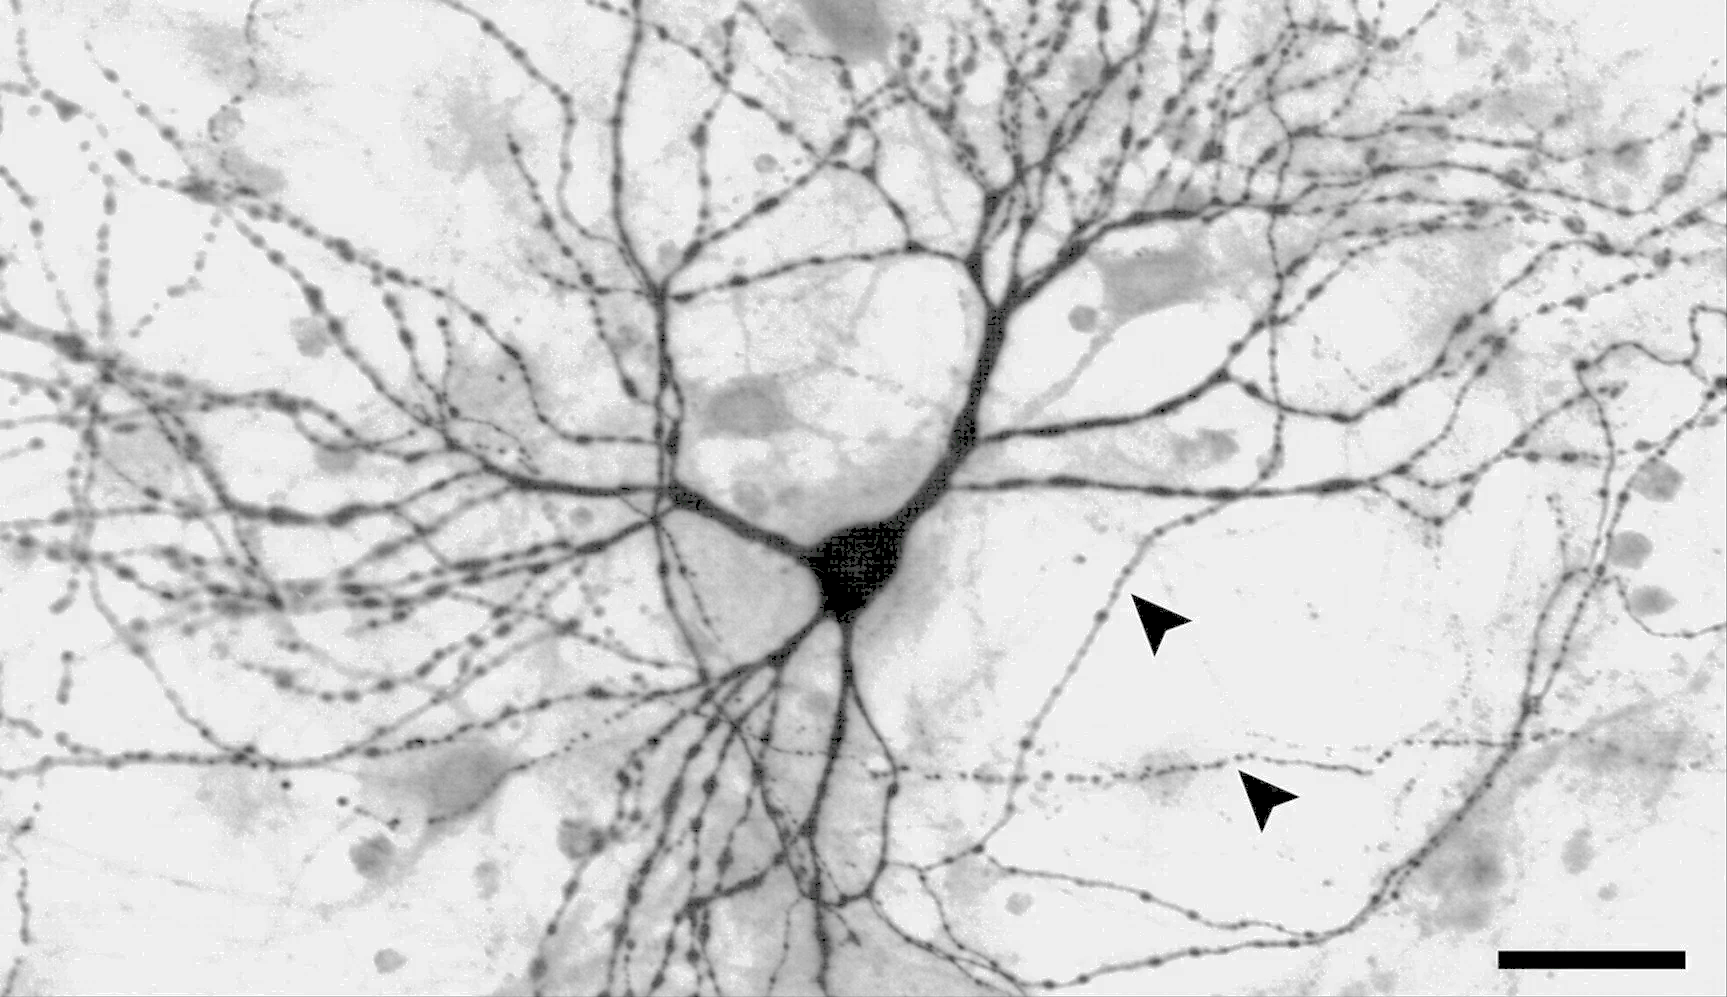
\includegraphics[width = 4 in]{brain_cells.png}
  \caption{ Image of a biological neural network by B. Zemelman et al -- https://doi.org/10.1073/pnas.242738899
}
\end{figure}



\end{document}









